\documentclass{article}
% --- watermark (auto-inserted) ---
\usepackage{xcolor}
\usepackage{xfp}% \fpeval; in the kernel since 2022, harmless on older LaTeX
\usepackage{draftwatermark}
\newlength{\watermarkTextWidth}
\AddToHook{begindocument/end}{%
  \SetWatermarkText{\normalfont Generated by The Agentic Scientist}%
  \SetWatermarkFontSize{10pt}%
  \SetWatermarkLightness{0.85}%
  \settowidth{\watermarkTextWidth}{\normalfont\fontsize{10pt}{12pt}\selectfont Generated by The Agentic Scientist}%
  \edef\watermarkScale{\fpeval{0.8 * sqrt(\paperwidth**2 + \paperheight**2) / \watermarkTextWidth}}%
  \edef\watermarkAngle{\fpeval{atand(\paperheight/\paperwidth)}}%
  \SetWatermarkScale{\watermarkScale}%
  \SetWatermarkAngle{\watermarkAngle}%
}
% --- end watermark ---
 % For LaTeX2e
\usepackage{paper,times}

\usepackage{hyperref}
\usepackage{url}
\usepackage{graphicx}
\usepackage{subcaption}
\usepackage{booktabs}
\usepackage{amsmath,amssymb,amsthm}

\newtheorem{proposition}{Proposition}

\title{Verified Minimal-Investment Planning for Leaderboard Rank Targeting under Multiple Aggregation Rules}
\iclrfinalcopy
\author{Anonymous authors}

\begin{document}
\maketitle

\begin{abstract}
Multi-task leaderboards turn a matrix of per-task scores into a single ranking through an aggregation rule, and a developer who can raise a target model's score on selected tasks, for example by training on related data, may be able to push it to first place. How much such targeted investment is needed, and how that quantity depends on the aggregation rule, is the question that motivates this work. We formalize targeted investment as non-negative, independent per-task score gains, priced either by total points (L1) or by the number of tasks touched (L0), with success meaning the target is strictly first under eight rules (mean, median, trimmed mean, z-score mean, Borda, plurality, Copeland, maximin). We then study a verification-first planner that returns the cheapest plan it can certify, combining exact solvers for four rules with verified heuristics for the others. On two held-out Open LLM Leaderboard boards, scored by a trusted evaluator against its own reference solver, the planner reaches a mean efficiency of 1.0032 relative to the reference, against 0.8166 for the better of two naive baselines, with every response well-formed; the evaluation is qualified. Because per-rule costs were not retained, we do \emph{not} test whether required investment varies across rules, and the results say nothing about real training effects.
\end{abstract}

\section{Introduction}
Multi-task benchmarks are the standard instrument for comparing machine-learning models: a leaderboard collects scores of many models on many sub-datasets and an aggregation rule, most often the arithmetic mean, converts each model's score vector into a rank \citep{Hendrycks2020MeasuringMM,Liang2022HolisticEO}. Rankings influence adoption, publication and funding, so developers have an incentive to act on them, which is the familiar pattern in which a metric used as a target ceases to measure what it was meant to measure \citep{Thomas2020RelianceOM}. One class of actions is to include data related to some of the sub-datasets in a model's training, which raises its scores on those tasks. Prior work documents that leaderboards are sensitive to task selection \citep{Dehghani2021TheBL}, to aggregation choices \citep{Colombo2022WhatAT,Rofin2022VotenRankRO,Lanctot2023EvaluatingAU}, to private testing and uneven sampling \citep{Singh2025TheLI}, and to benchmark leakage \citep{Zhou2023DontMY,Sainz2023NLPEI,Yang2023RethinkingBA}. What remains less examined is a quantitative, rule-by-rule account of how large a targeted investment must be for a specific model to reach first place.

This paper takes a first, deliberately narrow step: it makes the question computable and checks that the computation can be done reliably. We (i) define a declared investment model and two cost measures, (ii) specify eight aggregation rules and the strict-first success criterion, and (iii) study a planner whose every output is re-verified against an exact replica of the rule before it is returned. The planner is assessed on held-out public leaderboard snapshots by an evaluator that owns the rule engine, the plan verifier, a reference solver, naive baselines and control conditions; candidate-reported diagnostics are never trusted.

\paragraph{What the evidence supports.} The held-out evaluation completed and is qualified: the planner's main efficiency exceeds that of the naive baselines and all integrity checks passed. The measured quantity is \emph{cost-efficiency of the planner relative to an evaluator-owned reference solver} under the declared investment model. It is not a measurement of how much investment real developers need, and the retained metrics contain no per-rule or per-target cost tables. The hypothesis that minimal required investment varies with the aggregation rule therefore remains a motivating hypothesis here, neither supported nor refuted.

\paragraph{Contributions.}
\begin{itemize}
\item A formal targeted-investment model for multi-task leaderboards with L1 (points) and L0 (task count) costs, a field definition, and a strict-first success criterion covering eight aggregation rules (Section~\ref{sec:setup}).
\item A verification-first planner (exact solvers for mean, median, maximin and plurality; verified heuristics for trimmed mean, z-score mean, Borda and Copeland; plan verification, pruning, boundary polishing and a safe fallback) whose design is documented at the level of the evaluated source (Section~\ref{sec:planner}).
\item A held-out evaluation on two Open LLM Leaderboard boards against a reference solver, naive baselines and two controls, with a separate development comparison of three planner configurations on HELM MMLU (Section~\ref{sec:results}).
\item An explicit statement of what is \emph{not} established, including rule-dependence of required investment, generalization to other boards, and any statistical significance beyond two evaluator seeds (Section~\ref{sec:limits}).
\end{itemize}

\begin{figure}[t]
\centering
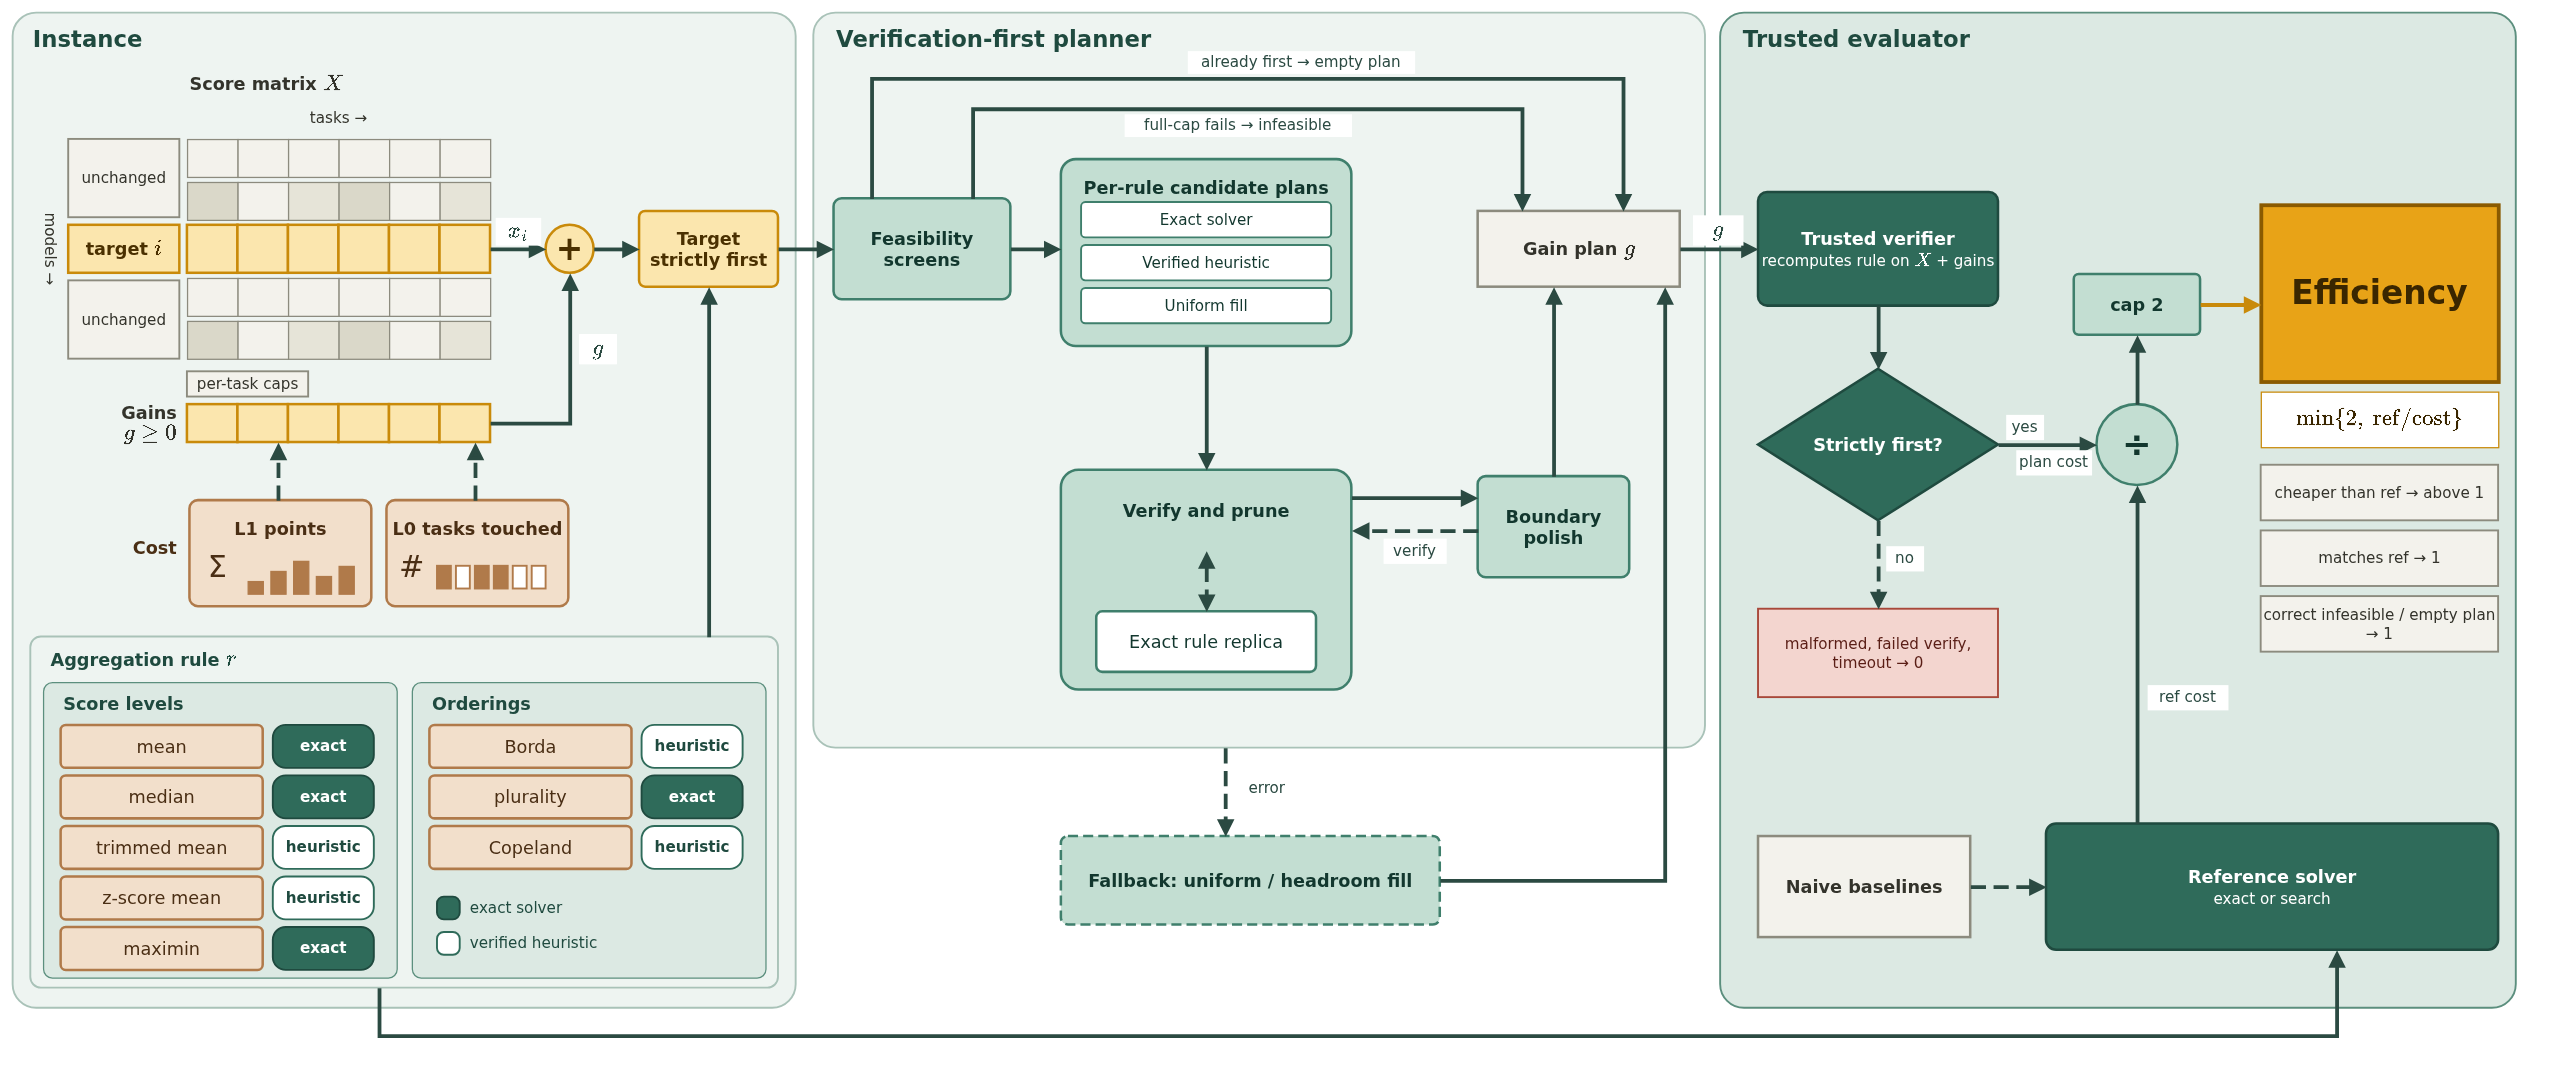
\includegraphics[width=\textwidth]{figures/overview_schematic.png}
\caption{Overview. A public score matrix, an investment model (independent non-negative per-task gains with L1 or L0 cost), and an aggregation rule define an instance in which a target model must become strictly first. A planner proposes a gain plan; a trusted verifier recomputes the rule on the modified matrix; efficiency is the cost of the evaluator's reference plan divided by the cost of the verified plan, capped at 2.}
\label{fig:overview}
\end{figure}

\section{Related Work}
\paragraph{Multi-task benchmarks and their aggregation.} Broad suites such as MMLU, its hard BIG-bench subset and HELM summarize models by averaging over many sub-tasks \citep{Hendrycks2020MeasuringMM,Suzgun2022ChallengingBT,Liang2022HolisticEO}. The Open LLM Leaderboard \citep{OpenLLMLeaderboardContents2025}, whose public snapshot supplies our held-out boards, aggregates six benchmarks \citep{Zhou2023InstructionFollowingEF,Suzgun2022ChallengingBT,Hendrycks2021MeasuringMP,Rein2023GPQAAG,Sprague2023MuSRTT,Wang2024MMLUProAM}. Critiques show that the mean is a modeling choice with consequences: task choice can reorder methods \citep{Dehghani2021TheBL}, leaderboard design embeds assumptions about user utility \citep{Ethayarajh2020UtilityII}, and aggregate statistics need uncertainty-aware treatment \citep{Agarwal2021DeepRL}. Social-choice formulations replace the mean with voting rules for models, agents or systems \citep{Colombo2022WhatAT,Rofin2022VotenRankRO,Lanctot2023EvaluatingAU}. We use that rule family not to recommend a rule but as the set of aggregators over which a targeted-investment cost is defined.

\paragraph{Leaderboard gaming and contamination.} Evidence of strategic behavior includes selective private testing and uneven data sampling on the Chatbot Arena platform \citep{Chiang2024ChatbotAA}, as analyzed by \citet{Singh2025TheLI}, training on evaluation data \citep{Zhou2023DontMY}, per-benchmark contamination measurement \citep{Sainz2023NLPEI}, and paraphrased test items that evade decontamination \citep{Yang2023RethinkingBA}. Adaptive reuse of a holdout is a related validity threat \citep{Dwork2015TheRH}. A game-theoretic treatment of benchmark designers and developers who post-train strategically is given by \citet{Chen2026LeaderboardIM}. Our setting is complementary and simpler: a single actor, a fixed public matrix, and a computed cost of a hypothetical intervention, with no equilibrium analysis and no model of how training data transfers across tasks.

\paragraph{Computational social choice.} Manipulation, bribery and margin-of-victory problems ask how little must change for a chosen candidate to win under a voting rule \citep{Bartholdi1989TheCD,Faliszewski2006HowHI,Xia2012ComputingTM,Conitzer2016BarriersTM}. The closest discrete analogues price the intervention: bribery models give each voter a price for changing their vote \citep{Faliszewski2006HowHI}, and swap bribery charges for each exchange of adjacent candidates in a voter's ranking \citep{Elkind2009SwapB}. Complexity results depend on the rule and on tie-breaking; for example, Copeland voting has been studied for its resistance to bribery and control \citep{Faliszewski2009LlullAC}, and tie-breaking conventions change manipulation complexity \citep{Obraztsova2011TiesMC}. We cite these results as context only: we do not prove hardness for the planner's problems and do not claim that the planner's heuristics inherit any of these guarantees. Our problem is a continuous variant: the ``voters'' are tasks, the intervention changes one candidate's scores (not preferences directly), and cost is measured in score points or in touched tasks. We borrow the strict-win convention, under which ties count against the target.

\section{Problem Setup and Method}\label{sec:setup}

\subsection{Targeted investment on a leaderboard}
A leaderboard is a matrix $X\in[0,100]^{N\times T}$ of scores of $N$ models on $T$ tasks (higher is better). An aggregation rule $r$ maps $X$ to a vector $v^r(X)\in\mathbb{R}^N$. A developer controls a target row $i$ and can choose gains $g\in\mathbb{R}^T_{\ge 0}$, replacing $x_i$ by $x_i+g$ while leaving every other row unchanged; there is no spillover across tasks and no effect on other models. Gains are bounded by per-task caps $c_t$, so $g_t\le c_t-x_{it}$. Two cost measures are used:
\begin{align}
\text{L1 (points):}\quad & \mathrm{cost}(g)=\textstyle\sum_t g_t, && c_t=100,\\
\text{L0 (breadth):}\quad & \mathrm{cost}(g)=|\{t: g_t>0\}|, && c_t=\max_j X_{jt}+10^{-6}.
\end{align}
Under L0 each targeted task is lifted at most to the best score in the field on that task, so breadth cost measures \emph{how many tasks must be treated}, not how far. \emph{Success} means that the target is strictly first after modification, recomputed by the evaluator with a margin of $10^{-9}$ so that ties count against the target. The \emph{field} is the top $\min(N,200)$ fully observed models by arithmetic mean, and \emph{targets} are the models at mean-rank 2 and mean-rank 10. The planning problem is
\begin{equation}
\min_{g}\ \mathrm{cost}(g)\quad\text{s.t.}\quad v^r_i(X+e_i g^\top)>\max_{j\neq i}v^r_j(X+e_i g^\top),\ \ 0\le g_t\le c_t-x_{it},
\end{equation}
and a correct report of infeasibility is also admissible. Section~\ref{sec:limits} discusses why each modeling choice is a restriction rather than a description of real training.

\subsection{Aggregation rules}
Table~\ref{tab:rules} lists the eight rules, with the planner's solution method from its source and the reference solver's method from the evaluator source. Mean, median, trimmed mean (dropping the lowest and highest 20\% of tasks), maximin (worst-task score) and z-score mean (per-task standardization recomputed on the modified matrix) act on score levels; Borda (mean per-task rank), plurality (number of tasks on which a model is strictly first) and Copeland (pairwise task-majority wins) act on per-task orderings and are piecewise constant in $g$. Raising the target's own scores can only help it under all rules except z-score mean, because that rule re-standardizes each column using the modified matrix and so can move rivals' values in either direction; the planner's source treats it as non-monotone.

\begin{table}[t]
\centering
\caption{Aggregation rules and solution methods (from the evaluated sources). ``Exact'' refers to the method documented in the source, up to the numerical margin; it is not independently proven here.}
\label{tab:rules}
\small
\begin{tabular}{@{}p{2.3cm}p{1.7cm}p{3.25cm}p{3.0cm}@{}}
\toprule
Rule & Acts on & Planner & Reference solver\\
\midrule
mean & levels & closed form (exact) & exact threshold plan\\
median & levels & order-statistic enumeration (exact for L0 and uniform-cap L1) & exact threshold plan for odd $T$; search otherwise\\
maximin & levels & lift all tasks below best rival's minimum (exact) & exact threshold plan\\
trimmed mean (20\%) & levels & floor plans with bisection, then pruning; L0 greedy with restarts & search\\
z-score mean & levels, non-monotone & floor plans and steepest ascent; L0 greedy & search with continuous polish\\
Borda & orderings & hull-greedy over tasks (L1); greedy with restarts (L0) & level-table family and greedy\\
plurality & orderings & per-count rival quotas, cheapest-first (exact) & level-table family and greedy\\
Copeland & orderings & level-move ratio greedy (L1); greedy (L0) & level-table family and greedy\\
\bottomrule
\end{tabular}
\end{table}

\paragraph{Conceptual cost structure (not measured here).} Some structure follows directly from the definitions. Under the mean, the L1 cost of success is exactly $T$ times the gap between the best rival's mean and the target's mean, up to the margin, whenever the headroom suffices, and the L0 cost is the smallest number of tasks whose headroom covers that total (Appendix~\ref{app:model}). Under maximin, cost is governed entirely by the tasks on which the target is below the best rival's worst score. Under plurality the target must become the unique leader on each treated task, and rivals that lose their only wins add further requirements. These statements motivate the hypothesis that required investment differs across rules; they are derived from the definitions, not tested on leaderboard data in this paper.

\subsection{Design rationale and hypotheses}
Three considerations shaped the planner, and each yields a hypothesis that the evaluation can address in part.
\emph{Verification before return.} Discrete rules flip at exact floating-point ties, and heuristics that shave a plan to the boundary can land on the wrong side by rounding. Returning only plans that an exact replica of the rule confirms removes this failure mode at the cost of extra evaluations, and it makes the planner's output trustworthy independently of the solver that proposed it. \emph{Rule-specific structure.} A uniform gain ignores which tasks are cheap to lift; solvers that exploit the structure of each rule (Table~\ref{tab:rules}) should find cheaper plans than a rule-agnostic fill. \emph{Boundary polishing.} A plan returned by a constructive heuristic is rarely tight, so shrinking each gain to the verification boundary, dropping redundant tasks and moving points between tasks should lower cost further, and for L0 two-for-one swaps can reduce the number of treated tasks. We state three hypotheses:
\begin{description}
\item[H1 (planner advantage).] The frozen verified planner (base solvers, verification, pruning and boundary polishing) has higher main efficiency than the better of the evaluator's uniform-gain and greedy marginal-cost baselines on held-out boards. The held-out study evaluates the planner as a whole, so H1 does not isolate the per-rule solvers from verification, pruning, polishing or the uniform-gain fallback.
\item[H2 (polish).] Boundary polishing lowers verified plan cost relative to the base solvers on a development leaderboard.
\item[H3 (MILP selection).] A MILP level-selection layer lowers cost for the discrete rules (Borda, Copeland, plurality) and the trimmed mean relative to the base solvers.
\end{description}
H1 is the only hypothesis tested on held-out data. H2 and H3 are tested only in the development comparison with two seeds. The question of rule-dependence in required investment is not among the tested hypotheses (Section~\ref{sec:results}).

\subsection{Verification-first planner}\label{sec:planner}
The evaluated planner answers each instance within a per-episode time budget (5\,s internal solve budget; the evaluator allows 12\,s per episode). Its design is conservative: no plan is returned that has not been re-applied to the matrix and re-scored by an exact replica of the rule.
\begin{enumerate}
\item \textbf{Feasibility screens.} If the target is already first the plan is empty. For monotone rules, if even the full-cap plan fails, the instance is reported infeasible; for z-score mean a steepest-ascent search is tried first because the full-cap plan need not be best.
\item \textbf{Per-rule candidate plans.} Exact solvers are used for mean, median, maximin and plurality; verified heuristics (floor-family plans, convex-hull and ratio greedy, restarted greedy for L0) for trimmed mean, z-score mean, Borda and Copeland (Table~\ref{tab:rules}). A uniform-gain plan (L1) or headroom-ordered fill (L0) is always added as a candidate.
\item \textbf{Verification and pruning.} Each candidate is verified; for non-exact rules, coordinate-wise bisection (L1) or task dropping (L0) removes redundancy as long as success is preserved.
\item \textbf{Boundary polishing.} A time-boxed (2\,s) loop on the cheapest verified plan performs per-task bisection to the verification boundary, drops redundant tasks, and applies pairwise transfers between tasks (a ladder of step sizes for L1, two-for-one swaps for L0). A polished plan replaces the original only if it verifies and costs no more.
\item \textbf{Fallback.} Any internal error falls back to the uniform-gain or headroom-fill routine of the starter code.
\end{enumerate}
The source also contains offline helpers (bootstrap intervals, paired tests, task subsampling) that the response handler never calls; they were not used to produce any reported number.

\subsection{Evaluation protocol}\label{sec:protocol}
The evaluator owns the rule engine, the plan verifier, the reference solver, the naive baselines and the controls. The \emph{episode efficiency} of a verified successful plan is $\min\{2,\,\max(\mathrm{ref},\epsilon)/\max(\mathrm{cost},\epsilon)\}$, where $\mathrm{ref}$ is the reference solver's cost and costs below 0.01 points count as 0.01 (L0 costs are counts). A correct infeasibility claim, or a correct empty plan for an already-first target, scores 1; any other outcome, including malformed or timed-out responses, scores 0 and is never retried or dropped. The reference solver is exact for mean, maximin and odd-$T$ median and search-based otherwise, and its candidate set includes the polished naive baselines for L1; hence an average efficiency above 1 means the planner's verified plans were on average slightly cheaper than the reference plans, not that the reference is optimal.

\emph{Main efficiency} averages over boards, over main cases (8 rules $\times$ 2 targets $\times$ 2 cost measures per board) and over evaluator seeds. \emph{Control efficiency} averages two conditions per board and rule: a permuted-input control (non-identity row and task permutations, reference cost invariant) and a within-task shuffled-score null (columns shuffled across models, target set to the rank-2 model of the shuffled matrix, own reference). \emph{Plan validity rate} is the fraction of declared episodes with a well-formed in-bounds response. The \emph{combined} score is $0.8\times$main $+\,0.2\times$control. The naive baselines (uniform gain and greedy marginal-cost) are scored against the same reference, taking the better of the two per case. A held-out evaluation is \emph{qualified} when integrity checks pass, main efficiency strictly exceeds the baseline's, and (when time permits) a replayed first episode reproduces its verified cost.

\paragraph{Data and splits.} Development uses the 57 HELM MMLU v1.13.0 subject columns as tasks. The held-out evaluation uses two boards built from the Open LLM Leaderboard snapshots \citep{OpenLLMLeaderboardContents2025}: a six-benchmark board from the \texttt{contents} table and a sub-task-level board from the \texttt{results} files for the same model pool, each restricted to the top $\min(N,200)$ models. The evaluator verifies snapshot checksums and checks that the held-out boards are disjoint from the development data. Development seeds are 11 and 12; held-out seeds are 9001 and 9002.

\paragraph{Compared configurations.} The held-out study evaluates one frozen planner: base solvers plus boundary polishing. For a development-only component comparison, three configurations were scored on HELM MMLU: the base solvers (Base); the base solvers with an additional MILP level-selection layer for Borda, Copeland, plurality and trimmed mean and an exchange polish for z-score L0 (Base+MILP); and the base solvers with boundary polishing (Base+Polish). The Base+Polish source does not contain the MILP layer, so these are alternative extensions of the base rather than a cumulative chain. Only Base+Polish was carried into the held-out study. No development-plane baseline metric was retained.

\section{Results}\label{sec:results}

\subsection{Held-out evaluation}
\begin{figure}[t]
\centering
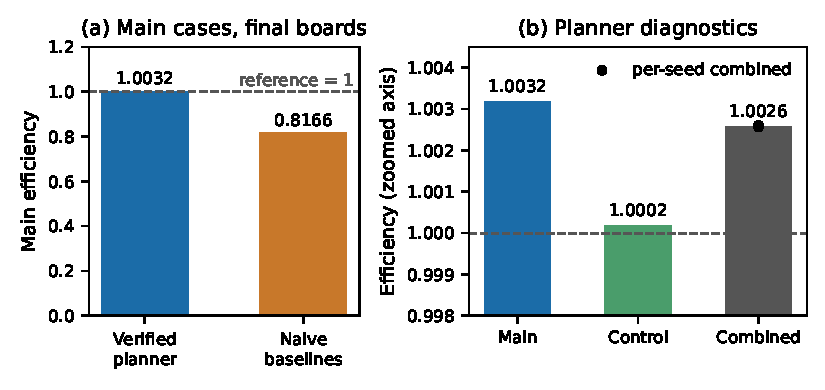
\includegraphics[width=\textwidth]{figures/final_efficiency_comparison.pdf}
\caption{Held-out evaluation on two Open LLM Leaderboard boards (two evaluator seeds). (a) Main efficiency of the verified planner and of the better of two naive baselines per case, against the reference level of 1. (b) Main, control and combined efficiency of the planner on a zoomed axis; dots are the two per-seed combined values.}
\label{fig:final}
\end{figure}

The held-out evaluation completed and its outcome is qualified. The planner's main efficiency is 1.0032 relative to the reference solver, % @evidence[[paper_data.json#final_evaluation.metrics.main_efficiency]]
versus 0.8166 for the better naive baseline per case, % @evidence[[paper_data.json#final_evaluation.metrics.baseline_main_efficiency]]
a difference of 0.187 (Figure~\ref{fig:final}a). The plan validity rate is 1.0, % @evidence[[paper_data.json#final_evaluation.metrics.plan_validity_rate]]
so no episode was malformed, timed out or out of bounds. Control efficiency is 1.0002, % @evidence[[paper_data.json#final_evaluation.metrics.control_efficiency]]
and the combined score is 1.0026. % @evidence[[paper_data.json#final_evaluation.metrics.combined_score]]
Per-seed combined scores were 1.00260 and 1.00257 for seeds 9001 and 9002, % @evidence[[paper_data.json#final_evaluation.evaluation_evidence.episodes]]
and each seed individually satisfies the gate that main efficiency exceeds the baseline's.

Three observations bound the interpretation. First, an efficiency near 1 means that the planner's verified plans cost, on average, about the same as the reference plans; the retained value does not reveal how many cases sit exactly at 1, how many are above, or whether any case is below. Second, the planner's candidate set includes the uniform-gain and headroom-fill plans, and the comparison is between the whole frozen planner (base solvers, verification, pruning, boundary polishing and the uniform-gain fallback) and the evaluator's naive baselines. No held-out ablation separates the per-rule solvers from those other components, so the gap of 0.187 cannot be attributed to the solvers specifically (in development, polishing alone moved main efficiency from 1.0031 to 1.0051). The comparison also does not show that this planner is better than other sophisticated planners, which were not evaluated. Third, the two evaluator seeds do not resample the leaderboard: they change permutation and shuffle draws and restart randomness, so the 3.5$\times10^{-5}$ spread between seeds reflects solver and control variability, not data sampling, and no confidence interval or significance test can be formed from two values.

\paragraph{Reading an efficiency near 1.} The held-out main efficiency averages 64 main cases per seed (8 rules, 2 target ranks, 2 cost measures, 2 boards), each with weight $1/64\approx0.0156$. An excess of 0.0032 over 1 is therefore about one fifth of the credit a single case would add at the maximal per-episode efficiency of 2, and about 0.2 of a case-unit in total. The retained aggregate cannot distinguish many tiny savings relative to the reference from a few larger savings offset by some losses; this decomposition is unknown.

\subsection{Controls and diagnostics}
The retained mean control efficiency is 1.0002, so on average the planner's efficiency relative to the evaluator's references on the permuted-input and shuffled-null cases was close to 1. This aggregate cannot show per-case cost agreement: savings on some cases and losses on others may offset, and no per-case or per-condition control records were retained. On the development leaderboard the controls averaged 0.9967 for all three configurations, so control plans there did not simply match their references. The controls are designed to check invariance to row and task order and non-vacuity of the instance; the retained aggregate does not establish that they were passed, and they do not probe whether the planner overfits the Open LLM boards. The evaluator recomputes every plan's validity and cost itself; candidate-reported diagnostics are marked unverified in the retained evidence and were not used.

\subsection{Component comparison on the development leaderboard}
\begin{figure}[t]
\centering
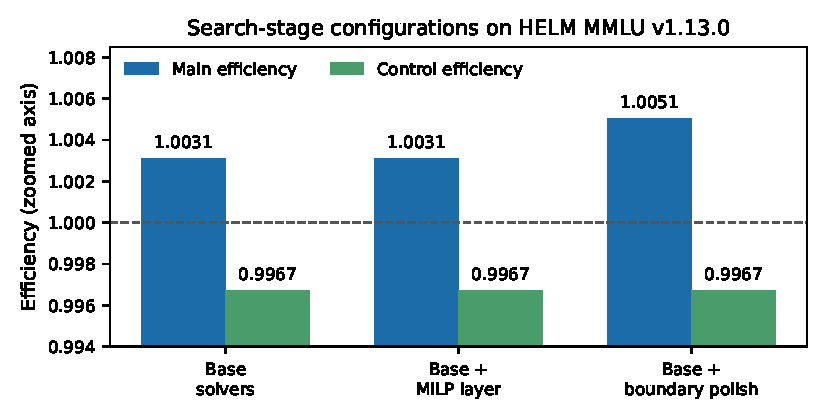
\includegraphics[width=\textwidth]{figures/search_variant_comparison.pdf}
\caption{Development comparison on HELM MMLU v1.13.0 (two seeds each). Differences between configurations are in the third decimal; the axis is zoomed accordingly. Control efficiency is 0.9967 for all three.}
\label{fig:search}
\end{figure}

On HELM MMLU, Base and Base+MILP have identical combined scores (1.00183) and identical main efficiency (1.0031), % @evidence[[source_evidence/search_metrics/config_01_metrics.json#main_efficiency]]
so the MILP layer and exchange polish produced no measured change; whether it never found a cheaper verified plan or the heuristics already matched it is not recoverable from the retained evidence. Base+Polish reaches main efficiency 1.0051 % @evidence[[source_evidence/search_metrics/config_03_metrics.json#main_efficiency]]
and combined score 1.00339, an increase of 0.0016 in combined score over Base (Figure~\ref{fig:search}). % @evidence[[paper_data.json#all_programs]]
The two seeds of each configuration agree to within $3\times10^{-6}$ in combined score, which shows reproducibility of the evaluator's computation for a fixed matrix but is not a test of the configuration difference. Control efficiency is 0.9967 for Base and Base+MILP and 0.9967 for Base+Polish, % @evidence[[source_evidence/search_metrics/config_03_metrics.json#control_efficiency]]
and every configuration has plan validity 1.0. Per-seed evaluator wall-clock was about 9\,s for Base, 24--25\,s for Base+MILP and 35--37\,s for Base+Polish (Appendix Table~\ref{tab:search}), so the polish's small gain in cost is bought with roughly four times the compute at evaluation.

Taken together with the held-out value, main efficiency was 1.0051 for the selected configuration on HELM MMLU and 1.0032 on the held-out boards. This is a descriptive observation about two different leaderboards, not evidence of transfer or of generalization.

\subsection{Status of the hypotheses}
\begin{table}[t]
\centering
\caption{Evidential status of the hypotheses and of the motivating question. ``Not measured'' means no retained metric addresses the statement.}
\label{tab:status}
\small
\begin{tabular}{@{}p{3.3cm}p{1.9cm}p{4.0cm}@{}}
\toprule
Statement & Status & Evidence and scope\\
\midrule
H1: frozen planner beats naive baselines & Supported for the whole planner & Held-out main efficiency 1.0032 vs.\ 0.8166; two boards, two seeds; no held-out ablation isolates the per-rule solvers; pool includes the naive plan\\
H2: polish lowers cost & Small gain, unreplicated & Development combined 1.00339 vs.\ 1.00183; two seeds; about 4$\times$ evaluator wall-clock\\
H3: MILP layer lowers cost & Not supported & Development metrics identical to base; cause not recoverable\\
Required investment varies by rule & Not measured & No per-rule costs retained\\
Generalization to other boards or real training & Not measured & Outside the declared model\\
\bottomrule
\end{tabular}
\end{table}

\subsection{What these results do not show}
The retained metrics contain no per-rule, per-target or per-cost-measure breakdown, no infeasibility counts, and no correlation analysis against the shuffled null. We therefore make no claim about which aggregation rule is most or least costly to manipulate, about how cost depends on target rank, or about whether L0 and L1 costs disagree. Missing diagnostics are unknown, not negative.

\section{Discussion and Limitations}\label{sec:limits}
\paragraph{Scope of the claim.} The qualified outcome certifies that, under the declared investment model and on two held-out boards, the verified planner was more cost-efficient than naive baselines and returned well-formed plans throughout. Qualification is a gate defined by the evaluator; it does not establish generalization to other leaderboards, field sizes or targets, nor does it speak to real training.

\paragraph{Investment model.} Independent per-task gains without spillover contradict how training data usually behaves: data for one task often helps related ones, a contamination effect discussed in \citet{Zhou2023DontMY} and \citet{Sainz2023NLPEI}. Uniform costs, whether per point or per task, ignore that some tasks are cheaper to improve. The cap policy (100 for L1, field-best for L0) and the field definition (top 200 by mean, targets at ranks 2 and 10) are choices, and sensitivity to them was not measured. Treating a target as fixed also ignores that rivals could respond, which is the setting of \citet{Chen2026LeaderboardIM}.

\paragraph{Reference and baselines.} The reference solver is exact only for some rules, so efficiency is relative, not optimal; a value above 1 is possible and was observed on average. Efficiency is capped at 2 per episode, which bounds the influence of individual cases, and costs under 0.01 points are floored, which hides tie-breaking differences. The planner was not compared with generic integer-programming or black-box optimization baselines other than the MILP variant on the development data.

\paragraph{Statistics.} Two evaluator seeds on two boards that share a model pool, and two seeds on one development leaderboard, are the only variability evidence. Differences among configurations in the third decimal should be read as descriptive. Candidate-reported diagnostics are unverified.

\paragraph{What a rule-dependence test would require.} Answering the motivating question needs paired, per-case costs rather than efficiencies: for each board, target rank and cost measure, the reference (or planner) cost under every rule, including infeasible cases as censored outcomes rather than zeros. Rule effects would then be summarized with bootstrap intervals over targets and compared with paired rank tests with multiplicity correction; the shuffled-score null would indicate how much of any difference comes from the correlation structure of real task scores rather than from the rule itself; and sensitivity to the field size, the cap policy and the target rank would be reported as robustness checks. The planner source contains offline helpers for the interval and test computations, but none of them was run to produce a reported number.

\paragraph{Coupling between planner and evaluator.} The planner's internal rule replica implements the same definitions that the task specifies and that the evaluator's rule engine uses, so agreement between the two on whether a plan succeeds is by construction; the evaluator nevertheless recomputes every plan with its own independent code, and a disagreement would have scored zero. The retained evidence does not report any such disagreement, but it also does not break out failure counts, other than the plan validity rate of 1.0, which only covers well-formedness.

\paragraph{Dual use.} A tool that finds cheap rank-lifting interventions could support gaming of leaderboards. We view it instead as a diagnostic for benchmark designers: an aggregation rule whose rank is cheaply reachable by few-task interventions is a warning sign, though this paper does not measure that for any rule.

\section{Conclusion}
We formalized targeted investment on multi-task leaderboards and evaluated a verification-first planner that returns only plans re-checked against an exact replica of the aggregation rule. On two held-out Open LLM Leaderboard boards, the planner's mean efficiency relative to an evaluator-owned reference solver was 1.0032, against 0.8166 for the better naive baseline, with a plan validity rate of 1.0 and a qualified outcome. A development comparison on HELM MMLU suggests that boundary polishing improves cost slightly (combined 1.00339 versus 1.00183 for the base solvers) at higher compute, whereas an additional MILP level-selection layer (with a z-score exchange polish) changed nothing measurable. These conclusions are conditional on the declared investment model, rest on two evaluator seeds, and concern planner cost-efficiency. The central question that motivated the study, how much required investment varies with the aggregation rule, needs per-rule, per-target cost tables with paired uncertainty and the shuffled-null comparison; these remain future work, as do models with spillover and heterogeneous task costs.

\paragraph{Reproducibility statement.} The planner sources, the evaluator sources, the task contract and the script that builds each figure are included with the submission (Appendix~\ref{app:repro}). Data snapshots are identified by revision hash and file checksums. All reported numbers are read from evaluator outputs.

\paragraph{Ethics statement.} The work uses only public leaderboard scores and trains no models. Dual-use considerations are discussed above.

% IMPORTANT: \clearpage flushes all pending floats before references so that
% body-page counting excludes reference-only pages.  Do NOT remove.
\clearpage
\bibliography{references}
\bibliographystyle{paper}

\clearpage
\appendix
\section{Supplementary Information}

\subsection{Investment model, rules and elementary cost identities}\label{app:model}
\paragraph{Instance definition.} An instance is a tuple $(X,i,r,\text{cost model})$ with $X\in[0,100]^{N\times T}$ restricted to the field, a target row $i$, a rule $r$ from Table~\ref{tab:rules}, and L1 or L0 costs. Per-task headroom is $h_t=c_t-x_{it}$. Rule definitions follow the evaluator's rule engine: Borda scores are minus the mean per-task rank (ties share half credit), plurality counts tasks on which a model is the unique maximizer, Copeland counts pairwise task-majority wins with half credit for ties, and the trimmed mean drops $\lfloor T/5\rfloor$ tasks from each end. The main cases are the 32 combinations of rule, target rank (2, 10) and cost measure per board; control cases use rank 2 and L1 for each of the 8 rules, once for the permuted input and once for the shuffled null.

\begin{proposition}[Mean and maximin]
Let $\Delta=\max_{j\ne i}\bar x_j-\bar x_i$ with $\bar x$ the row mean, and $m^\star=\max_{j\neq i}\min_t x_{jt}$. Under the mean, an L1 plan succeeds iff $\sum_t g_t>T\Delta$, so the infimum cost is $T\Delta$ (attained up to the margin) provided $\sum_t h_t>T\Delta$; the L0 cost is the smallest $k$ such that the $k$ largest headrooms sum to more than $T\Delta$. Under maximin, success requires $\min_t(x_{it}+g_t)>m^\star$, so the L1 infimum is $\sum_t\max(0,m^\star-x_{it})$ and the L0 cost is $|\{t:x_{it}\le m^\star\}|$, subject to the caps.
\end{proposition}
\emph{Proof sketch.} The mean of the modified row is $\bar x_i+\sum_t g_t/T$ and rivals are unchanged, which gives the first claim; allocation across tasks is irrelevant for L1, and for L0 the cheapest set of tasks is the one with the largest headroom. For maximin, every task with $x_{it}\le m^\star$ must be lifted above $m^\star$ and no other task needs to move. \hfill$\square$

These identities are elementary consequences of the definitions and agree with the closed forms documented in the planner source; they are not used to produce any reported number. The remaining rules lack comparably simple identities, which is why the planner relies on verified search.

\subsection{Full retained metrics}
\begin{table}[h]
\centering
\caption{Held-out metrics from the sealed final evaluation (Open LLM Leaderboard boards).}
\label{tab:final}
\small
\begin{tabular}{@{}lr@{}}
\toprule
Metric & Value\\
\midrule
Main efficiency (planner) & 1.0031855 \\ % @evidence[[paper_data.json#final_evaluation.metrics.main_efficiency]]
Main efficiency (better naive baseline per case) & 0.8165814 \\ % @evidence[[paper_data.json#final_evaluation.metrics.baseline_main_efficiency]]
Control efficiency & 1.0001938 \\ % @evidence[[paper_data.json#final_evaluation.metrics.control_efficiency]]
Plan validity rate & 1.0000000 \\ % @evidence[[paper_data.json#final_evaluation.metrics.plan_validity_rate]]
Combined score ($0.8\,$main$+0.2\,$control) & 1.0025871 \\ % @evidence[[paper_data.json#final_evaluation.metrics.combined_score]]
Seed 9001: combined score / duration & 1.0026048 / 31.4\,s \\ % @evidence[[paper_data.json#final_evaluation.evaluation_evidence.episodes]]
Seed 9002: combined score / duration & 1.0025695 / 33.0\,s \\ % @evidence[[paper_data.json#final_evaluation.evaluation_evidence.episodes]]
Qualification: status / outcome & completed / qualified \\ % @evidence[[paper_data.json#final_evaluation.outcome]]
\bottomrule
\end{tabular}
\end{table}

\begin{table}[h]
\centering
\caption{Development comparison on HELM MMLU v1.13.0. Durations are per-seed evaluator wall-clock (seeds 11, 12).} % @evidence[[paper_data.json#all_programs]]
\label{tab:search}
\small
\begin{tabular}{@{}lrrrrr@{}}
\toprule
Configuration & Main & Control & Combined & Validity & Duration (s)\\
\midrule
Base solvers & 1.0031 & 0.9967 & 1.00183 & 1.0 & 9.3, 8.8\\ % @evidence[[source_evidence/search_metrics/config_01_metrics.json]]
Base + MILP layer & 1.0031 & 0.9967 & 1.00183 & 1.0 & 25.0, 23.7\\ % @evidence[[source_evidence/search_metrics/config_02_metrics.json]]
Base + boundary polish & 1.0051 & 0.9967 & 1.00339 & 1.0 & 37.3, 34.8\\ % @evidence[[source_evidence/search_metrics/config_03_metrics.json]]
\bottomrule
\end{tabular}
\end{table}

\subsection{Planner components}
The evaluated source has three layers. (i) \emph{Exact replica.} \texttt{verify\_ranks\_first} re-applies the gains to the target row and recomputes the rule on the full matrix; a margin of $2\times10^{-8}$ is demanded locally, above the evaluator's $10^{-9}$. (ii) \emph{Candidates.} Per-rule solvers, plus the starter uniform plan, are verified, pruned and sorted by cost. (iii) \emph{Polish.} Up to six passes of shrink, drop and pairwise-transfer moves are applied within 2\,s, and the result is accepted only if verified and not costlier. The MILP variant, evaluated on the development leaderboard only, adds a level-selection integer program (with a 4\,s solver budget per episode) whose plan is accepted only after verification, so it can only tie or improve on the heuristic plan; the retained scores are identical to Base. Implementation details come from the included source files \texttt{source\_evidence/planner\_boundary\_polish\_source.py}, \texttt{planner\_milp\_variant\_source.py} and \texttt{planner\_base\_source.py}.

\subsection{Data provenance and reproducibility}\label{app:repro}
\paragraph{Data.} Development: HELM MMLU release v1.13.0 (summary date 2025-01-10), 57 subject files, exact-match column, each file pinned by SHA-256 in the task manifest. Held-out: Open LLM Leaderboard \texttt{contents} at revision \texttt{9c09a7cae43334062a82cb164f2ef255013dafa2} (parquet SHA-256 \texttt{f13a7061\ldots dca5}) and \texttt{results} at revision \texttt{aa81ecc38fdc5708254b833923368970efdf5ef5} (derived sub-task file SHA-256 \texttt{c4536f9f\ldots 4a7f}). Flagged models and rows with missing values are excluded, and a newer submission replaces an older duplicate. Licenses: no dataset-level license is declared for the score data; the HELM code is Apache-2.0; \texttt{contents} carries per-model Hub license fields. Use is limited to research analysis of published scores.

\paragraph{Software and runs.} Python with NumPy 2.5.4, SciPy 1.18.1 and PyArrow 26.0.1, CPU only. Development seeds 11, 12; held-out seeds 9001, 9002. Per-seed held-out evaluator wall-clock was 31.4 and 33.0\,s. Held-out outcome identifiers: evaluator SHA-256 \texttt{02531dad\ldots e163e}, planner source tree \texttt{db5d072f\ldots d4734f} (hashes identify provenance and are not evidence of correctness). The figure script \texttt{scripts/build\_figures.py} regenerates Figures~\ref{fig:final} and~\ref{fig:search}; Tables~\ref{tab:final} and~\ref{tab:search} are transcriptions of retained metric files.

\paragraph{Not done.} No per-rule experiment, sensitivity analysis over $K$, caps or targets, spillover model, or comparison with additional planners was performed; no confidence intervals were computed.

\subsection{LLM Usage}
An LLM-based autonomous research system carried out the work reported here, including problem formalization, planner implementation, evaluation runs and the drafting of this manuscript. The held-out numbers were produced by the evaluator, and every reported value is read from retained evaluator outputs. Literature references were retrieved through public bibliographic APIs, and cited works were not read in full by the system beyond their abstracts and metadata.

\end{document}
